 \documentclass[handout,nooutcomes,noauthor,hints]{ximera}

\graphicspath{  
{./}
{./whoAreYou/}
{./drawingWithTheTurtle/}
{./bisectionMethod/}
{./circles/}
{./anglesAndRightTriangles/}
{./lawOfSines/}
{./lawOfCosines/}
{./plotter/}
{./staircases/}
{./pitch/}
{./qualityControl/}
{./symmetry/}
{./nGonBlock/}
}


%% page layout
\usepackage[cm,headings]{fullpage}
\raggedright
\setlength\headheight{13.6pt}


%% fonts
\usepackage{euler}

\usepackage{FiraMono}
\renewcommand\familydefault{\ttdefault} 
\usepackage[defaultmathsizes]{mathastext}
\usepackage[htt]{hyphenat}

\usepackage[T1]{fontenc}
\usepackage[scaled=1]{FiraSans}

%\usepackage{wedn}
\usepackage{pbsi} %% Answer font


\usepackage{cancel} %% strike through in pitch/pitch.tex


%% \usepackage{ulem} %% 
%% \renewcommand{\ULthickness}{2pt}% changes underline thickness

\tikzset{>=stealth}

\usepackage{adjustbox}

\setcounter{titlenumber}{-1}

%% journal style
\makeatletter
\newcommand\journalstyle{%
  \def\activitystyle{activity-chapter}
  \def\maketitle{%
    \addtocounter{titlenumber}{1}%
                {\flushleft\small\sffamily\bfseries\@pretitle\par\vspace{-1.5em}}%
                {\flushleft\LARGE\sffamily\bfseries\thetitlenumber\hspace{1em}\@title \par }%
                {\vskip .6em\noindent\textit\theabstract\setcounter{question}{0}\setcounter{sectiontitlenumber}{0}}%
                    \par\vspace{2em}
                    \phantomsection\addcontentsline{toc}{section}{\thetitlenumber\hspace{1em}\textbf{\@title}}%
                     }}
\makeatother



%% thm like environments
\let\question\relax
\let\endquestion\relax

\newtheoremstyle{QuestionStyle}{\topsep}{\topsep}%%% space between body and thm
		{}                      %%% Thm body font
		{}                              %%% Indent amount (empty = no indent)
		{\bfseries}            %%% Thm head font
		{)}                              %%% Punctuation after thm head
		{ }                           %%% Space after thm head
		{\thmnumber{#2}\thmnote{ \bfseries(#3)}}%%% Thm head spec
\theoremstyle{QuestionStyle}
\newtheorem{question}{}



\let\freeResponse\relax
\let\endfreeResponse\relax

%% \newtheoremstyle{ResponseStyle}{\topsep}{\topsep}%%% space between body and thm
%% 		{\wedn\bfseries}                      %%% Thm body font
%% 		{}                              %%% Indent amount (empty = no indent)
%% 		{\wedn\bfseries}            %%% Thm head font
%% 		{}                              %%% Punctuation after thm head
%% 		{3ex}                           %%% Space after thm head
%% 		{\underline{\underline{\thmname{#1}}}}%%% Thm head spec
%% \theoremstyle{ResponseStyle}

\usepackage[tikz]{mdframed}
\mdfdefinestyle{ResponseStyle}{leftmargin=1cm,linecolor=black,roundcorner=5pt,
, font=\bsifamily,}%font=\wedn\bfseries\upshape,}


\ifhandout
\NewEnviron{freeResponse}{}
\else
%\newtheorem{freeResponse}{Response:}
\newenvironment{freeResponse}{\begin{mdframed}[style=ResponseStyle]}{\end{mdframed}}
\fi



%% attempting to automate outcomes.

%% \newwrite\outcomefile
%%   \immediate\openout\outcomefile=\jobname.oc
%% \renewcommand{\outcome}[1]{\edef\theoutcomes{\theoutcomes #1~}%
%% \immediate\write\outcomefile{\unexpanded{\outcome}{#1}}}

%% \newcommand{\outcomelist}{\begin{itemize}\theoutcomes\end{itemize}}

%% \NewEnviron{listOutcomes}{\small\sffamily
%% After answering the following questions, students should be able to:
%% \begin{itemize}
%% \BODY
%% \end{itemize}
%% }
\usepackage[tikz]{mdframed}
\mdfdefinestyle{OutcomeStyle}{leftmargin=2cm,rightmargin=2cm,linecolor=black,roundcorner=5pt,
, font=\small\sffamily,}%font=\wedn\bfseries\upshape,}
\newenvironment{listOutcomes}{\begin{mdframed}[style=OutcomeStyle]After answering the following questions, students should be able to:\begin{itemize}}{\end{itemize}\end{mdframed}}



%% my commands

\newcommand{\snap}{{\bfseries\itshape\textsf{Snap!}}}
\newcommand{\flavor}{\link[\snap]{https://snap.berkeley.edu/}}
\newcommand{\mooculus}{\textsf{\textbf{MOOC}\textnormal{\textsf{ULUS}}}}


\usepackage{tkz-euclide}
\tikzstyle geometryDiagrams=[rounded corners=.5pt,ultra thick,color=black]
\colorlet{penColor}{black} % Color of a curve in a plot



\ifhandout\newcommand{\mynewpage}{\newpage}\else\newcommand{\mynewpage}{}\fi


\title{Roof area estimates}

\author{Bart Snapp and Claire Merriman}

\begin{document}
\begin{abstract}
 We make estimates with given measurements and start to determine what
 is, and is not, a reasonable estimate.
\end{abstract}
\maketitle

\begin{listOutcomes}
\item Know conventions and definitions to be used in later problems.
\item Distinguish between reasonable and unreasonable estimates.
\item Determine a reasonable estimate before preforming a calculation.
\end{listOutcomes}

\mynewpage
\begin{question}
Here are two shelters each with different roofs:
\begin{center}
  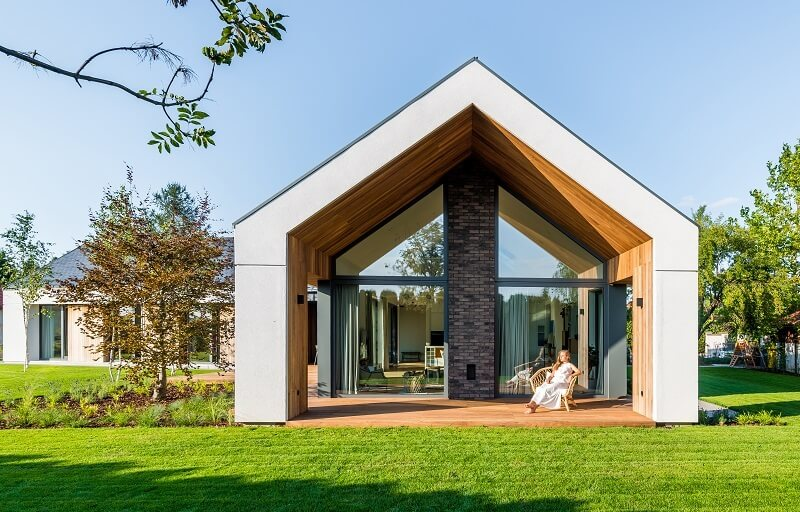
\includegraphics[height=.3\textwidth]{../formulasGalore/symRoof.jpg}\qquad 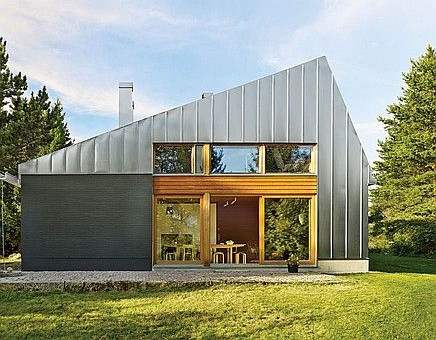
\includegraphics[height=.3\textwidth]{../formulasGalore/skewRoof.jpg}
\end{center}
  Below are diagrams of the roofs as seen from the top:
  \begin{center}
    \begin{tikzpicture}[x=1.5cm,y=1.5cm]
      \draw[ultra thick] (0,0) rectangle (3,2.4);
      %\draw[dashed] (.5,.5) rectangle (4.3,2.5);
    \draw[ultra thick] (0,1.2) -- (3,1.2);
    \draw[decoration={brace,raise=.2cm},decorate,thin] (0,0)--(0,2.4);
    \draw[decoration={brace,raise=.2cm,mirror},decorate,thin] (0,0)--(3,0);
    \node at (-.4,1.2) {$24'$};
    \node at (1.5,-.44) {$30'$};
    \node[above] at (1.5,1.2) {main ridge};
    \end{tikzpicture}
    \qquad
    \begin{tikzpicture}[x=1.5cm,y=1.5cm]
    \draw[ultra thick] (0,0) rectangle (5,3.6);
    %\draw[dashed] (.3,.3) rectangle (4.5,2.1);
    \draw[ultra thick] (0,3) -- (5,3);
    \draw[decoration={brace,raise=.2cm},decorate,thin] (0,0)--(0,3);
    \draw[decoration={brace,raise=.2cm,mirror},decorate,thin] (5,3.1)--(5,3.6);
    \draw[decoration={brace,raise=.2cm,mirror},decorate,thin] (0,0)--(5,0);
    \node at (-.5,1.5) {$30'$};
    \node at (5.4,3.3) {$6'$};
    \node at (2.5,-.44) {$50'$};
    \node[below] at (2.5,3) {main ridge};
  \end{tikzpicture}
  \end{center}
  You ask four friends what the surface areas of the two roofs
  are. They give you four different answers in each case. Here are
  their answers:
  \begin{center}
    \begin{tabular}{lll}
      Symmetrical Roof &\hspace{1in} & Asymmetrical roof\\
    \begin{minipage}{2in}\begin{enumerate}
    \item $9$ square feet
    \item $90$ square feet
    \item $900$ square feet
    \item $9000$ square feet
    \end{enumerate} 
    \end{minipage}
    & &
    \begin{minipage}{2in} \begin{enumerate}
    \item $20$ square feet
    \item $200$ square feet
    \item $2000$ square feet
    \item $20000$ square feet
      \end{enumerate}
    \end{minipage}
    \end{tabular}
  \end{center}
  Which answers above are \textbf{closest} to the correct answers?
  Explain how you arrive at your conclusions.
  \begin{freeResponse}
    \begin{enumerate}
    \item For the symmetrical roof, answer $(iii)$ is correct. The
      SMALLEST that the area of the roof could be is
      \[
      24\cdot 30 = 720.
      \]
      It is clear that the length of a side is around $12$ feet (half the width), so
      the LARGEST the are of the roof could be is
      \[
      \underbrace{720}_{\text{area of base}} + 2\cdot 12\cdot 30 = 1440.
      \]
      Note, $720 < 900 < 1440$.
    \item Answer $(iv)$ is correct.  The SMALLEST that the area of the
      roof could be is
      \[
      36\cdot 50 = 1800.
      \]
      The average of each side of the roof is a little greater than
      have of the width, so the LARGEST the are of the roof could be
      is
      \[
      \underbrace{1800}_{\text{area of base}} + 2\cdot 18\cdot 50 = 3600.
      \]
      Note, $1800 < 2000 < 3600$.
    \end{enumerate}
  \end{freeResponse}
\end{question}
\mynewpage

%% \begin{question}
%%  What additional information would you need to find the \textbf{actual} area of the roofs in the previous problem?
%% \end{question}
%% \mynewpage

\begin{question}
 As a gesture of friendship, Dr.\ Merriman has provided an outline of
 the house with the symmetrical roof with some measurements. Not all
 of these measurements are needed to find the area of the roof. You
 also need one additional measurement that was given in Problem 1.
 \begin{center}
  \begin{tikzpicture}[x=2.5cm,y=2.5cm]
    \draw[ultra thick] (0,0) -- (2.4,0);
    \draw[ultra thick] (0,0) -- (0,1);
    \draw[ultra thick] (2.4,0) -- (2.4,1);
    \draw[ultra thick] (1.2,1.9) -- (0,1);
    \draw[ultra thick] (1.2,1.9) -- (2.4,1);
    \draw[decoration={brace,raise=.2cm},decorate,thin] (0,0)--(0,1);
   \draw[decoration={brace,raise=.2cm,mirror},decorate,thin] (2.4,0)--(2.4,1.9);
    \draw[decoration={brace,raise=.2cm,mirror},decorate,thin] (1.15,1)--(1.15,1.9);
    \draw[decoration={brace,raise=.2cm,mirror},decorate,thin] (0,0)--(1.2,0);
    \draw[decoration={brace,raise=.2cm},decorate,thin] (2.4,0)--(1.2,0);
%    \draw[decoration={brace,raise=.2cm,mirror},decorate,thin] (1.2,1.9) -- (0,1);
%    \draw[decoration={brace,raise=.2cm},decorate,thin] (1.2,1.9) -- (2.4,1);
    \node at (-.25,.55) {$10'$};
    \node at (1.8,-.2) {$12'$};
    \node at (.6,-.2) {$12'$};
%    \node at (.5,1.6) {$15'$};
%    \node at (1.9,1.6) {$15'$};
    \node at (2.65,.95) {$19'$};
    \node at (1.4,1.45) {$9'$};
  \end{tikzpicture}
\end{center}
Calculate the surface area of the roof. How close is it to the
estimate from Problem 1?
\end{question}

\mynewpage

\begin{question}
 Dr.\ Merriman has also provided an outline of the house with the
 asymmetrical roof with some measurements. Not all of these
 measurements are needed to find the area of the roof. You also need
 one additional measurement that was given in Problem 1.
 \begin{center}
  \begin{tikzpicture}[x=2.5cm,y=2.5cm]
    \draw[ultra thick] (0,0) -- (3.6,0);
    \draw[ultra thick] (0,0) -- (0,1.125);
    \draw[ultra thick] (3.6,0) -- (3.6,1.125);
    \draw[ultra thick] (3,2.5) -- (0,1.125);
    \draw[ultra thick] (3,2.5) -- (3.6,1.125);
    \draw[decoration={brace,raise=.2cm},decorate,thin] (0,0)--(0,1.125);
    \draw[decoration={brace,raise=.4cm,mirror},decorate,thin] (3.6,0)--(3.6,2.5);
    \draw[decoration={brace,raise=.2cm,mirror},decorate,thin] (0,0)--(3,0);
    \draw[decoration={brace,raise=.2cm,mirror},decorate,thin] (3,0)--(3.6,0);
    \draw[decoration={brace,raise=.2cm,mirror},decorate,thin] (3,2.5) -- (0,1.125);
    \draw[decoration={brace,raise=.2cm},decorate,thin] (3,2.5) -- (3.6,1.125);
    \node at (-.4,.55) {$11.25'$};
    \node at (1.5,-.25) {$30'$};
    \node at (1.4,2) {$33'$};
    \node at (3.3,-.25) {$6'$};
    \node at (3.52,2) {$15'$};
    \node at (4,1.3) {$25'$};
  \end{tikzpicture}
\end{center}
 
 Calculate the surface area of the roof. How close is it to the
 estimate from Problem 1?
 
\end{question}
\end{document}
